\subsection{Supervised and unsupervised learning}
Derived from the different kinds of tabular data, we have two fundamental learning paradigms. Exemplary input data and possible results for both paradigms can be seen in \ref{fig:1_sv_vs_usv}.

\begin{figure}[h]
  \centering
  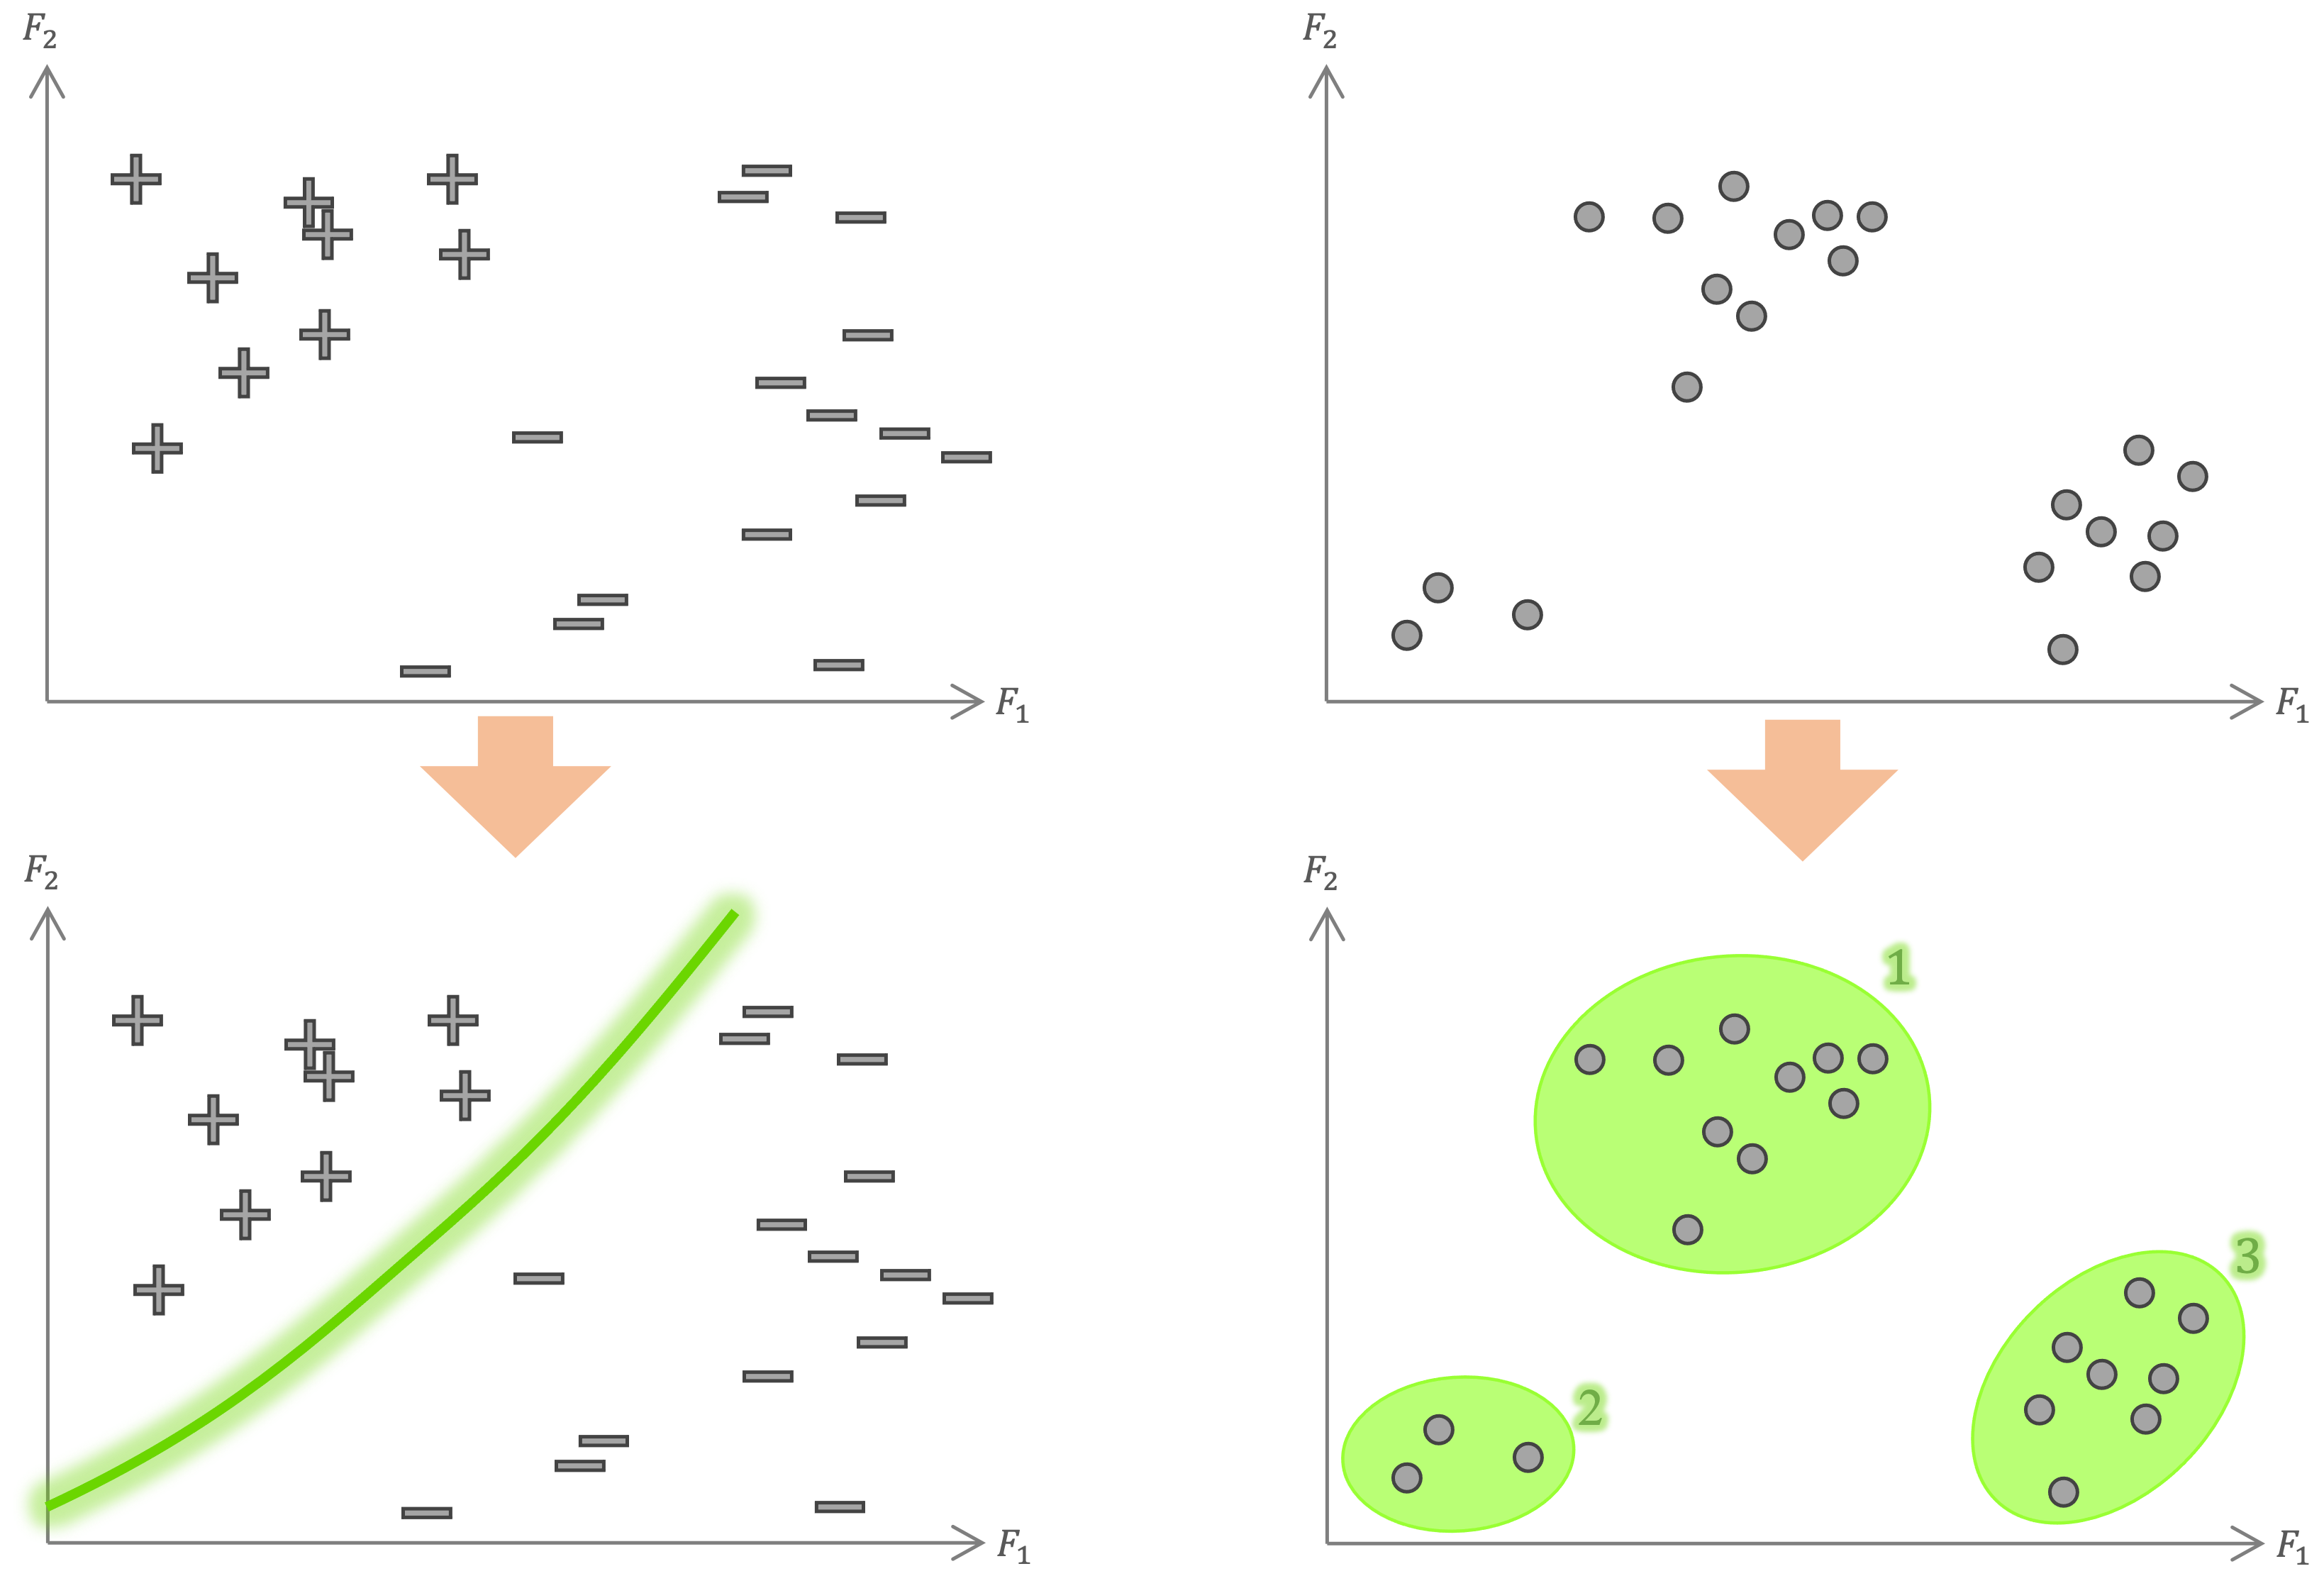
\includegraphics[width=0.6\textwidth]{assets/basics/SV_vs_US.png}
  \caption{Comparing supervised (left) and unsupervised (right) learning}
  \label{fig:1_sv_vs_usv}
\end{figure}

In the case of labeled data, we can apply \textbf{supervised learning}\sidenote{Supervised learning}. The goal is to find a "rule" in terms of descriptive features explaining the target feature as well as possible. \begin{note}Examples include:
\begin{itemize}
  \item Hospital environments where the target variable can be "recover" (yes or no), and the descriptive variables can be age, gender, smoking, $\dots$.
  \item University environments where the target variable can be "drops out" (yes or no), and the descriptive variables can be {\color{ForestGreen}mentor, prior education, $\dots$}.
  \item Production environments where the target variable can be "order is delivered in time" (yes or no), and the descriptive variables can be product, agent, $\dots$.
\end{itemize}\end{note}

In contrast to labeled data, we can also have instances without target labels, where we can only apply techniques of \textbf{unsupervised learning}\sidenote{Unsupervised learning}. The goal is to find clusters or patterns.
\begin{itemize}
  \item \textbf{Clusters}\sidenote{Cluster} are homogeneous sets of instances. \begin{note}Examples include finding similar groups of patients, students, customers, orders, cars, companies, and so on.\end{note}
  \item \textbf{Patterns}\sidenote{Pattern} on the other hand reveal hidden structures in the data, so basically the unknown unknowns. Rules of some form can be found in many environments. \begin{note}Examples can look like:
  \begin{itemize}
    \item Customers who buy bread and butter typically pay by phone.
    \item Patients who drink and smoke typically pay the hospital bill earlier than others.
    \item Products produced by team A on Monday tend to be returned more frequently by customers.
  \end{itemize}\end{note}
\end{itemize}

Interesting to regard is process discovery as a form of unsupervised learning in the way that a process model is just a very sophisticated rule. Important to mention, that this task can get very complex very quickly.
